\documentclass[11pt,a4paper]{article}
\usepackage[left=2cm,text={17cm,24cm},top=3cm]{geometry}
\usepackage[slovak]{babel}
\usepackage[]{opensans}
\usepackage[utf8]{inputenc}
\usepackage[T1]{fontenc}
\usepackage{times}
\usepackage{cite}
\usepackage{url}
\usepackage{color}
\usepackage[unicode,colorlinks,hyperindex,plainpages=false,urlcolor=black,linkcolor=black,citecolor=black]{hyperref}
\usepackage{graphics,picture}
\usepackage{listings}

\providecommand{\uv}[1]{\quotedblbase #1\textquotedblleft}

\clubpenalty=10000
\widowpenalty=10000

\begin{document}


%titlepage
\begin{titlepage}
\begin{center}
	\thispagestyle{empty}
	\textsc{\Huge Vysoké učení technické v~Brně\\[0.4em]
			\huge Fakulta informačních technologií}\\
	\vspace{\stretch{0.382}}
	{\LARGE 
	%Typografie a publikování\,--\,4. projekt\\[0.4em]
	Síťové aplikace a správa sítí\\[0.4em]
	\Huge 
	POP3 server}
	\vspace{\stretch{0.618}}
\end{center}
{\LARGE \today \hfill Peter Šuhaj}
\end{titlepage}	

%obsah
\setlength{\parskip}{0pt}

{\hypersetup{hidelinks}\tableofcontents}

\setlength{\parskip}{0pt}

\newpage

%text
\section{Úvod}
Táto dokumentácia popisuje program s názvom \textbf{popser} vytvorený ako projekt do predmetu Síťové aplikace a správa sítí. Úlohou tohoto zadania bolo vytvoriť e-mailový server, ktorý pracuje nad protokolom POP3, spracováva príkazy klientov a poskytuje na ne odpovede. Program má implementovať celú špecifikáciu POP3(okrem sekcie č. 8) a má pracovať s e-mailmy vo formáte IMF. V nasledujúcich častiach sú popísané jednotlivé protokoly, popis riešenia jednotlivých problémov a ich implementácia. 


\section{Dôležité pojmy}
Funkčnosť celej aplikácie je založená na niekoľkých protkoloch a štandardoch. K pochopeniu zadania a k vypracovaniu projektu je potrebné ich najprv preštudovať a porozumieť. 


\subsection{POP3}
Najdôležitejším protkolom v rámci celej implemetácie je protokol POP3(Post Office Protocol - Version 3) popísaný v RFC1939\cite{pop3}. Slúži na prístup k e-mailom na mailovom serveri ktorý podporuje tento protokol. Neposkytuje rozsiahle manipulačné operácie, zvyčajne klient sa pripojí k serveru, stiahne si maily a na serveri sa vymažú. Používa sa komunikácia klient-server. Klient po pripojení posielá príkazy serveru, server ich spracuje a poskytne odpoveď. Protokol popisuje presný formát správ a odpovedí. Odpoveď musí začať s +OK pri pozitívnej odpovedi, -ERR pri negatívnej. Pripojenie(session) prechádza niekoľkými stavmi. Obrázok \ref{fig:pop3FSM} popisuje stavy spojenia a prechody medzi nimi.

\begin{figure}[h]
  %\scalebox{0.4}{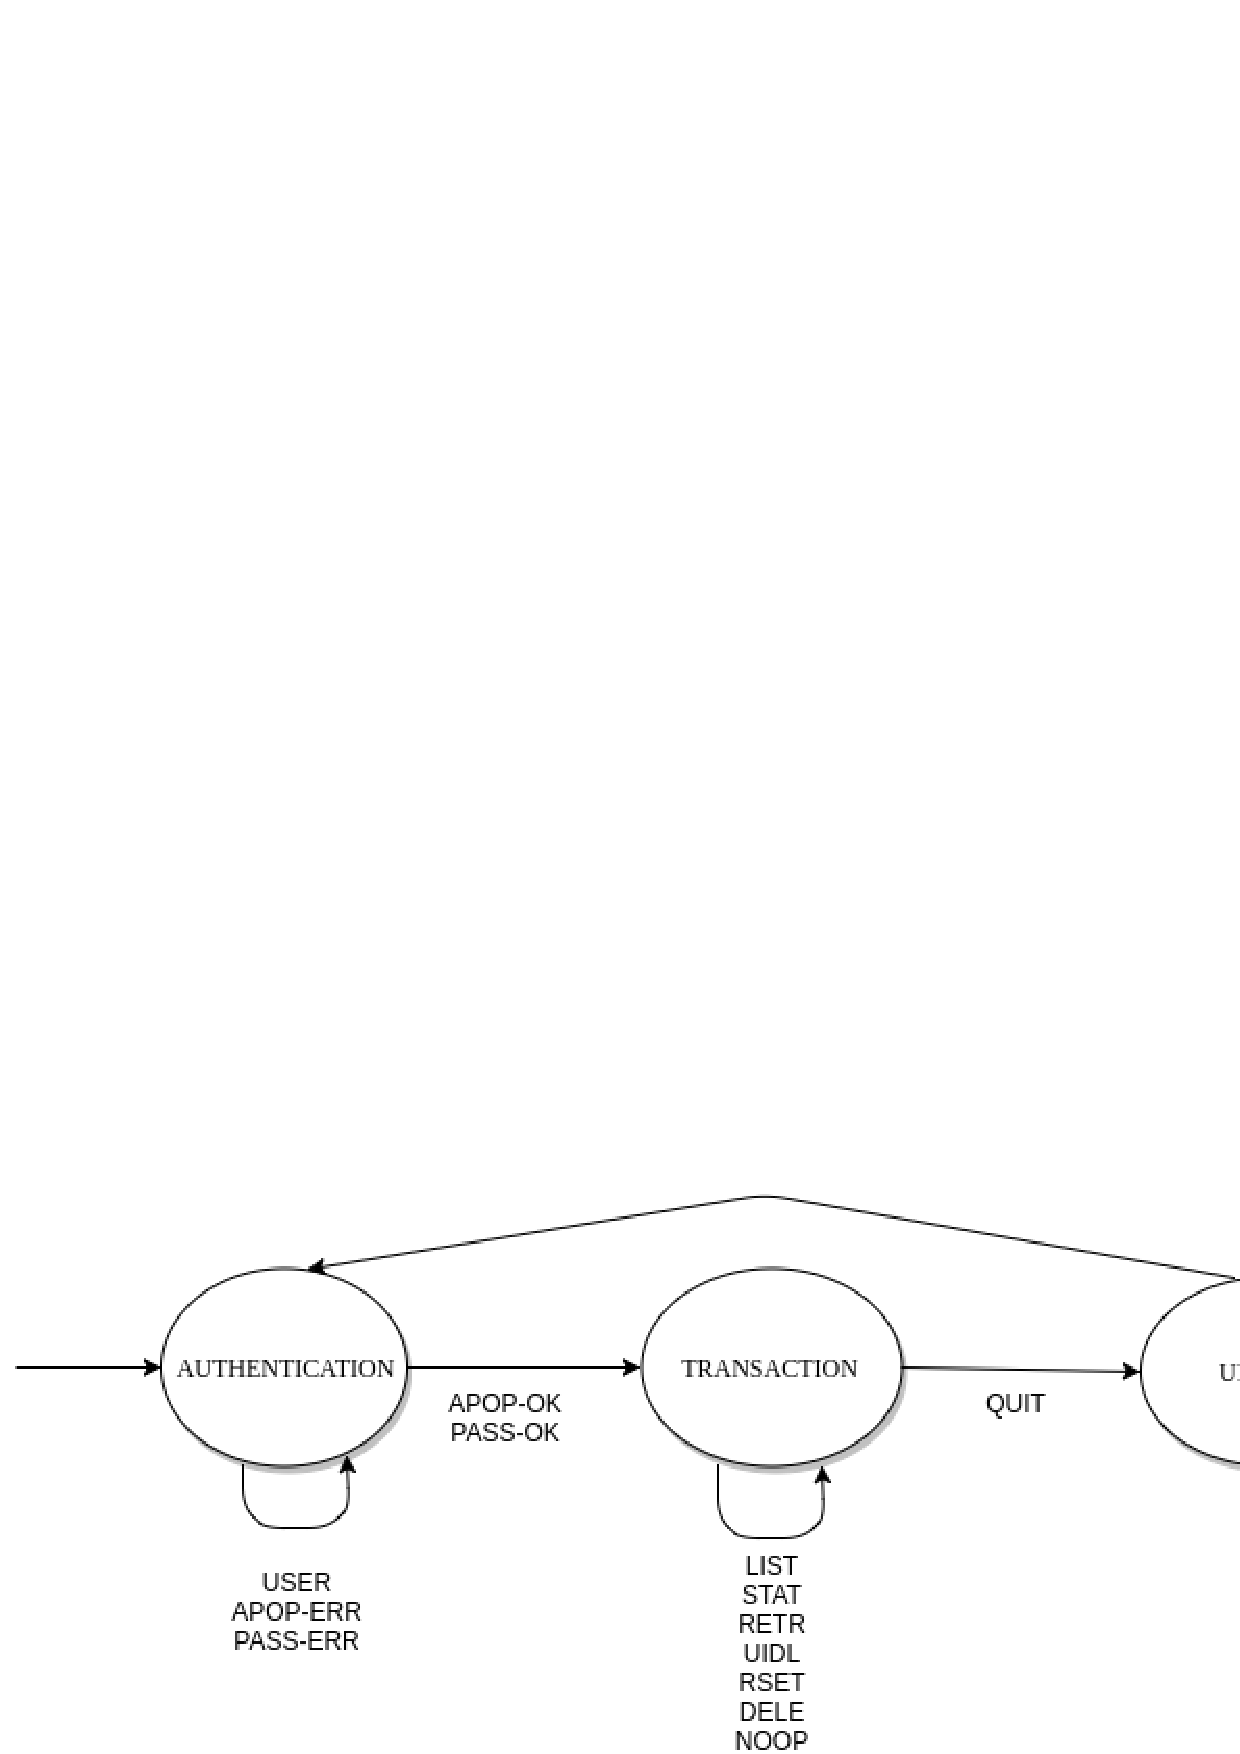
\includegraphics{pop3fsm.svg}}
  \scalebox{0.5}{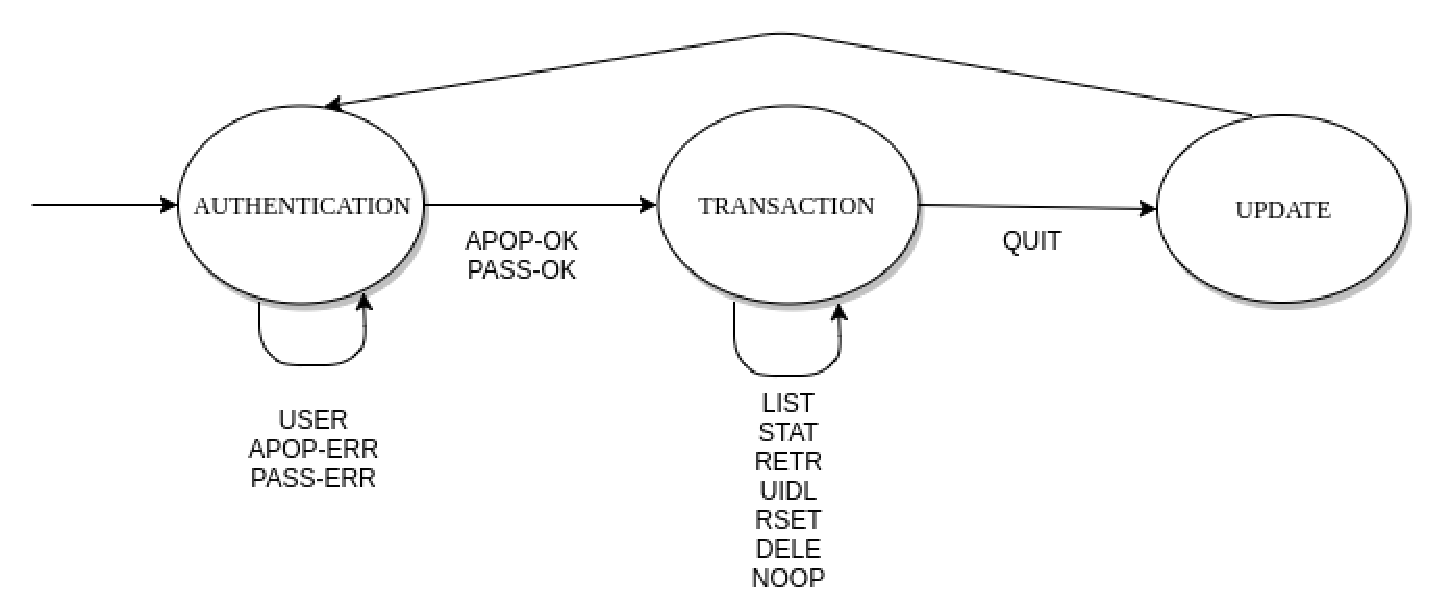
\includegraphics{pop3fsm.eps}}
  \centering
  \caption{Stavový automat pripojenia POP3.}
  \label{fig:pop3FSM}
\end{figure}


\subsection{IMF}
Internet message format je popísaný v RFC5322\cite{imf}. Udáva formát súborov s ktorými bude náš server pracovať. Každý e-mail sa má skladať z hlavičky a tela správy. Každý riadok súboru má byť ukončený s dvojicou znakou \textbackslash r\textbackslash n(tj. CRLF). 


\subsection{Maildir}
Formát Maildir\cite{maildir} popisuje potrebnú adresárovú štruktúru. Priečinok, ktorý bude použitý ako Maildir musí obsahovať adresáre \textbf{new}, \textbf{cur} a \textbf{tmp}, poprípade môže obashovať nejaké ďalšie súbory alebo adresáre. V rámci tejto implementácie sa používa iba new a cur, kedže s tmp pracujú rôzne SMTP servery. Tiež popisuje že jednotlivé e-mailové súbory musia mať jedinečný názov v rámci jedného Maildiru a premenovanie súborov pri presune z new do cur.\\\\




\section{Návrh a implementácia}
Program je implementovaný v jazyku C/C++ s použitím povolených knižníc potrebných pre vypracovanie zadania. Je rozdelený do dvoch modulov. Nie je použitý objektový návrh ale je vytvorená jedna trieda ktorý reprezentuje jeden modul. Druhý modul je hlavný program s funkciou main a s ostatnými potrenými funkciami.   

\subsection{Spracovanie argumentov}
Pre spracovanie argumentov bola vytvorená trieda \texttt{Arguments}, ktorá obsahuje privátne premenné pre každý prepínač a jednu metódu na kontrolu argumentov. Na začiatku sa kontroluje či bol zadaný prepínač -h. Ďalej sa kontroluje či bol program spustený iba so samotným prepínačom -r. Na koniec sa povienné a volitelné parametre kontrolujú pomocou funkcie \texttt{getopts} ktorá vyhodnotí správnosť parametrov a ich hodnôt. Na začiatku main sa vytvorí objekt typu Arguments a zavolá sa metoda na spracovanie argumentov.

\subsection{Pripojenie klientov}
Sieťová komunikácia a pripojenie klientov je riešená pomocou BSD socketov. Kedže sa jedná o server ktorý je paralelný, čiže paralelne vybavuje každé pripojenie boli použité vlákna z knižnice pthread.h. Keď sa jeden klient pripojí akceptuje sa pripojenie, vytvorí sa socket cez ktorý komunikuje a ďalej jeho požiadavky sú spracované v rámci vlákna. Túto časť popisuje ďalšia kapitola. Sockety sú nastavené ako neblokujúce.

\subsection{Spracovanie príkazov}

Táto časť implementácie je najrozsiahlejšia. Pre spracovanie príkazov pre každého klienta je vytvorené vlákno kde sa daný klient obsluhuje. Hlavnú čast tvorí smyčka kvôli použitiu nebolkojúceho socketu v ktorej je volaná funkcia recv, kontrolujú sa jej návratové hodnoty, prípadne či by blokovala. Po úspečnom načítaní dát do bufferu nasleduje spracovanie príkazov. Stavový automat ktorý je vidno na obrázku \ref{fig:pop3FSM} je implementovaný pomocou jazykovej konštrukcie switch, kde každý case repreyentuje jeden stav. C++ neumožňuje mať reťazce vo vetvách case, preto bola vytvorená enumerácia a pomocná funkcia, ktorá mapuje reťazce na odpovedajúce hodnoty enumerácie. Podobné riešenie bolo použíté pre spracovanie príkazov, ktoré sú spracované vo vstavoch. Výsledkom je dvojúrovňový switch, kde 1. úroveň udáva stav a 2. príkaz.

Ak sa príkaz spracoval a bol podporovaný nasleduje spracovanie prípadných argumentov. Pri príkazoch ktoré nemajú argument je možné zadať argument ale ten sa ignoruje. V prípadoch kde sú požadované argumenty tak sú povinné, ak nejaký chýba alebo je ich viac tak to server vyhodnotí ako chybu. Argumenty sa rozďelujú podľa medzier, výnimkou je príkaz PASS kde heslo môže obsahovať medzeru takže vlastne vždy bude mať iba jeden argument. Ak sa nepošle žiadny príkaz alebo poslaná správa nekončí dvojicou \textbackslash r\textbackslash n tak server pošle zápornú odpoveď klientovi.

Pre generovanie hashu pri príkazu APOP bola použitá funkcia \texttt{MD5} z knižnice \texttt{openssl/md5.h}. Táto funkcia bola tiež použitá pre vygenerovanie unikátneho identifikátoru pre súbory kde sa hashuje konkatenácia aktuálneho času, názvu súboru a globálna číselná premenná ktorá sa inkrementuje pri každom generovaní uidl.

Po úspešnej autentifikácii klienta je prevedná kontrola správnosti adresárovej štruktúry, ak je chybná tak server odpojí aktuálneho klienta. Tiež sa vykoná pokus o uzamknutie Maildiru. Pri tejto implementácií ak sa nepodarí pričinok uzamknúť tak klient je odpojený. Na uzamknutie sa používa globálna premenná typu \texttt{pthread\_mutex\_t}.    

Veľkosť súborov je vypočítaná pri presune z new do cur. Kvôli rôznej reprezentácií ukončovaniá riadku na odlišných systémoch bola potreba kontorlovať tento znak. V pŕipade ak riadok končí iba \textbackslash n tak k celkovej veľkosti je prirrátaný ešte jeden bajt, kedže protokol POP3 udává že každý riadok má byť ukončený \textbackslash r\textbackslash n. Výsledná veľkosť súboru sa teda skladá z fyzickej velkosti plus počet riadkov, ktoré boli ukončené iba s \textbackslash n.


Pri akejkoľvek internej chybe na serveri je vypísaná chybová hláška, klient je odpojený a vlákno sa skončí. 

\subsection{Ukončenie signálom SIGINT}
Na zachytenie signálu je použitá funkcia \texttt{signal} z knižnice \texttt{<csignal>}. Pri zachytení signálu je nastavená globálna premenná, ktorá sa kontroluje v podmienkách 
cyklu pre prijímanie pripojení vo funkcií main a pre komunikáciu s klientom vo funkcií pre vlákno. Táto kontorla je možná kvôli použitiu neblokujúcich socketov, kde sa cyklí. Vlákno ukončí socket na ktorom kommunikuje a vhodne sa ukončí. Funkcia main čaká na ukončenie každého vlákna. Táto časť je riešená pomocou globálnej premennej, kde sa ukladá aktuálny počet vlákien. Ak sa vytvorí vlákno tak premennú inkrementuje, pri ukončení dekrementuje. Funkcia main sleduje túto premennú a ak už nie je aktívne žiadne vlákno tak zatvorí pasívny socket a skončí program.

\subsection{Pomocné súbory, reset}
Kvôli fukcie reset, udil a kvôli tomu že obsah súboru okrem príkazov RETR a TOP môžeme čítať iba raz boli zavedené pomocné súbory. Jeden súbor s názvom log.txt obsahuje potrebné informácie o súboru vo formáte názov/uidl/filesize. Ako oddelovač bolo použité lomítko, ktoré nie je povolené v názve súboru na UNIXových systémoch takže jednoznačne sa dajú určiť kde jedna informácia končí a druhá začína. Súbor obsahuje pre každý e-mail jeden riadok. 

Do druhého súboru sú ukladané absolútne cesty všetkých e-mailov ktoré boli presunuté z new do cur. Pri zadaní prepínaču -r(reset) všetky súbory ktoré obsahuje súbor reset a sú fyzicky dostupné na disku sú presunuté z cur do new. Na konci sa všetky pomocné súbory vymažú.



\subsection{Použíté knižnice} 
\begin{lstlisting}
#include <iostream>
#include <cstdlib>
#include <string>
#include <string.h>
#include <unistd.h>
#include <netdb.h>
#include <sys/select.h>
#include <sys/socket.h>
#include <sys/types.h>
#include <sys/stat.h>
#include <netinet/in.h>
#include <arpa/inet.h>
#include <ctype.h>
#include <fstream>
#include <fcntl.h>
#include <openssl/md5.h>
#include <csignal>
#include <locale> 
#include <dirent.h>
#include <ctime>
#include <list>
#include <vector>
\end{lstlisting}


\section{Použitie programu}
Program má tri režimy behu:
\begin{enumerate}
  \item ./popser -h: Vypíše sa nápoveda, program sa správne ukončí.
  \item ./popser -r: Reset, Maildir sa vráti do stavu, ako keby server nebol nikdy spustení, program sa správne ukončí.
  \item ./popser -p číslo\_portu -a autentifikačný\_súbor -d  cesta\_k\_maildiru [-r] [-c]: Server sa spustí, komunikuje na zadanom porte, pracuje so zadaným Maildirom a načíta užívateľské meno a heslo zo súboru autentifikačný\_súbor. Pri zadaní parametru -c sa povolí autentifikácia typu USER/PASS, inak je povolená autentifikácia pomocou príkazu APOP. Parameter má rovnaký význam ako v príklade č. 2, čiže resetne server ale teraz sa neukončí ale beží ďalej.
\end{enumerate}



\section{Záver}
Program bol spočiatku vyvíjaný na Ubuntu 16.04.03 LTS, neskôr však radšej som to presunul na školský server Merlin kvôli tomu že tu sa bude testovať aj odovzdaná verzia.
Program je preložený prekladačom g++ a Makefile, ktorý je v odovzdaných súboroch. 


\newpage


%literatura
\makeatletter
%\def\@openbib@code{\addcontentsline{toc}{chapter}{Literatúra}}
\makeatother
\bibliographystyle{czechiso}

\begin{flushleft}
\bibliography{citace}
\end{flushleft}

\end{document}


